\chapter{Robot-Side Implementation}\label{chap:robot_side_rewrite}

Chapter~\ref{chap:system_architecture_rewrite} described the robot client as the embodied front end of the system.
This chapter describes the Pepper implementation.
The client runs as a NAOqi service, binds QiChat rules to Python methods, captures images, collects robot metadata, calls the server from Chapter~\ref{chap:server_side_rewrite}, speaks answers, and refreshes dynamic dialogue concepts.
The emphasis is the robot-side boundary: service methods, turn execution, grammar integration, metadata payloads, and development adapters.

\section{Runtime Structure}\label{sec:client-runtime-structure}

\begin{figure}[t]
\centering
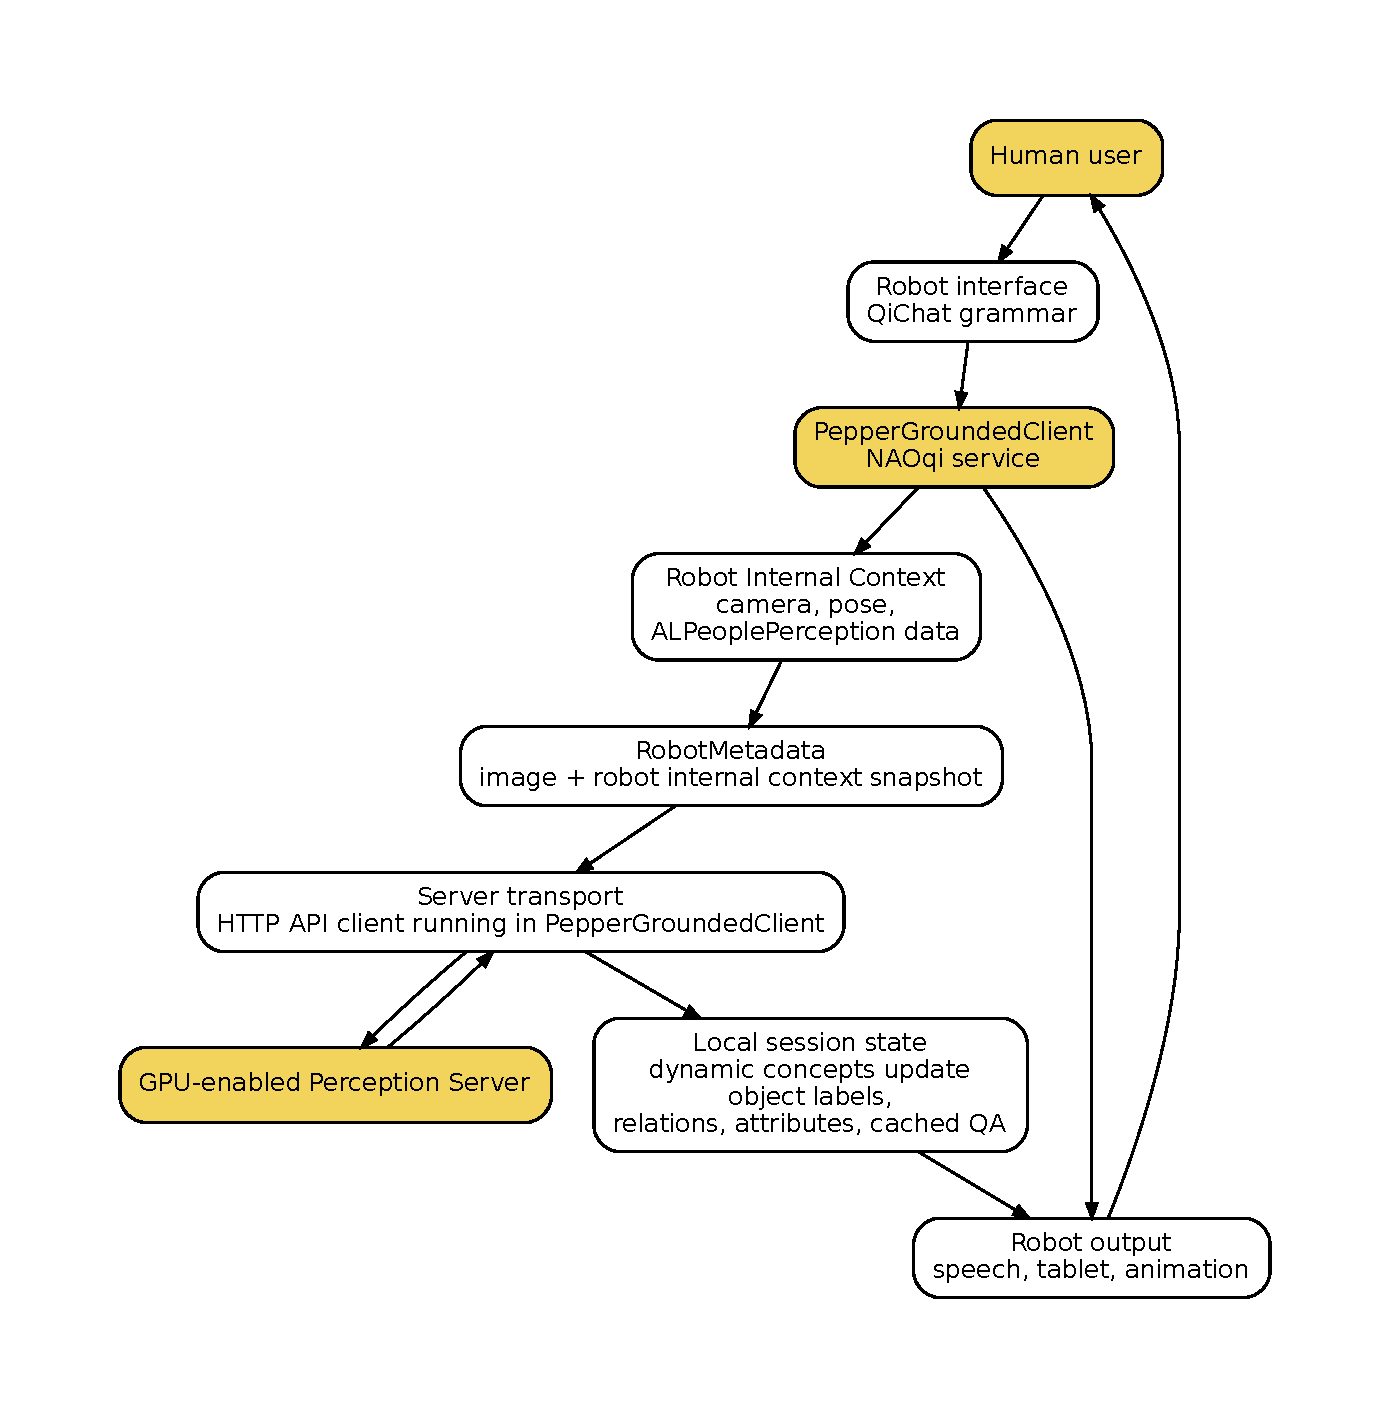
\includegraphics[width=\linewidth]{pics/client_clean_clean.pdf}
\caption[Robot-side client architecture.]{Robot-side client architecture. QiChat rules call bound methods of the robot client service. Long-running work is delegated to the turn manager, which coordinates capture, robot metadata, server communication, speech, local session state, and dynamic dialogue concepts.}
\label{fig:client-runtime-graph}
\end{figure}

Figure~\ref{fig:client-runtime-graph} shows the robot-side runtime.
The main Python service is registered in the NAOqi session under the name used by the QiChat topics.
After registration, a QiChat rule can call a bound method directly; for example, the quick-look intent starts a visual turn.
The service is kept as a thin boundary object.
It exposes methods for quick look, scan, chat, object-focused chat, cached answers, memory reset, configuration reload, and status inspection, while slow work is delegated to specialized components.

At startup, the service reads \texttt{client\_config.json} and constructs the client runtime.
The \texttt{SessionStore} keeps temporary local state such as the current chat identifier, last caption, remembered object labels, relation names, attributes, and cached question-answer pairs.
The \texttt{PepperServerTransport} owns HTTP communication with the server.
The camera, pose, people, face, social, sonar, speech, and dialog adapters wrap the corresponding NAOqi services.
The \texttt{Robot\-Con\-text\-Col\-lector} combines robot-native perception signals, and the \texttt{MetadataBuilder} turns those signals into the metadata payload sent with every visual request.
The \texttt{TurnManager} receives all these dependencies and implements the actual interaction workflows.

Adapters are practical on Pepper because NAOqi services differ in availability and failure behavior.
The physical robot provides \texttt{ALVideoDevice}; a virtual robot in Choregraphe does not reproduce the same camera behavior.
The implementation therefore includes \texttt{FakeCameraAdapter}, which reads frames from a local directory.
It is selected through \texttt{client\_config.json}, so the same turn manager can be tested locally and then run on the physical robot.

\section{QiChat Grammar and Service Binding}\label{sec:client-qichat}

The spoken interface is implemented with QiChat topics in English and Czech.
The topic files define the phrases that Pepper can recognize and map them to service calls.
QiChat therefore remains the deterministic action selector.
The VLM and LLM components are called only after the grammar has selected quick look, scan, object question, cached answer, or open chat.
This keeps the user-facing entry points predictable even when the server uses generative models downstream.

On the Python side, methods callable from QiChat are annotated with \texttt{@qi.bind}.
For example, \texttt{look(lang\_code)} and \texttt{scan(lang\_code)} are bound as public service methods and simply forward the request to \texttt{TurnManager.start\_look} or \texttt{TurnManager.start\_scan}.
This keeps the QiChat-facing method short.
The method logs the call, normalizes the minimal argument, and returns quickly, while the turn manager performs camera capture, server requests, speech, and memory refresh in a background thread.

\section{Dynamic Concepts and Scene-Aware Dialogue}\label{sec:client-dynamic-concepts}

Dynamic concepts are the main bridge from server-side scene memory back into robot speech recognition.
The English and Czech topics declare memory concepts for objects, attributes, relations, and cached questions.
They are not hard-coded lists in the topic files.
Instead, the client refreshes them from the server after perception updates, memory display, startup, and reset operations.

The refresh path starts with a call to the server memory summary endpoint.
The client stores the returned labels, label counts, scene graph edges, and pregenerated question-answer pairs in local session state.
Unary scene graph edges, where subject and object are the same instance, are treated as attributes.
Other edges are treated as relations.
The \texttt{DialogAdapter} then writes cleaned and capped values into ALDialog through \texttt{setConcept}.
Only compact recognition values are mirrored to the robot.
The full scene graph and object instances remain on the server, where grounding and memory reasoning are implemented.

As a result, the grammar changes with the perceived scene.
If the server has recently detected a \texttt{chair}, a \texttt{bottle}, and a \texttt{laptop}, the object-focused rule can begin to recognize questions about those labels without changing the topic file.
The same mechanism also enables cached question recognition from pregenerated questions in local session state.

\section{Turn Management}\label{sec:client-turn-management}

The operational center of the client is \texttt{TurnManager}.
Every slow action is exposed as a \texttt{start\_*} method.
When a service method calls one of these methods, the turn manager creates a turn identifier, checks a busy flag, optionally speaks an acknowledgement, and starts a daemon thread.
The original QiChat or tablet call can then return quickly instead of blocking the NAOqi service while the robot captures images or waits for the server.

The busy flag is a simple but important part of the implementation.
Pepper should not start two camera captures, head scans, speech actions, or memory refreshes at the same time.
If a new long-running turn arrives while another turn is active, the turn manager rejects it and speaks a localized busy fallback.
All guarded turns clear the busy flag in a \texttt{finally} block.
This prevents a camera error, timeout, malformed server response, or unexpected exception from leaving the robot permanently locked.

The turn manager also records latency events.
The logged milestones cover turn start, server request start, server response receipt, and speech start.
These timestamps are not needed for normal dialogue, but they are useful for the response-time measurements in Chapter~\ref{chap:experiment}.
They also make the role of acknowledgement utterances explicit.
An acknowledgement can begin immediately, reducing awkward silence, while the actual server request is executed in the background.

\section{Quick Look and Panorama Scan}\label{sec:client-visual-actions}

The quick-look action is optimized for a fast first spoken response.
The client captures one JPEG frame, collects robot metadata, and calls the server caption endpoint.
The request can also ask the server to run detection in the background.
Pepper can therefore speak a short caption as soon as the server returns it, while the server continues updating detections, scene graph relations, memory, and later dynamic concepts.

\begin{figure}[t]
\centering
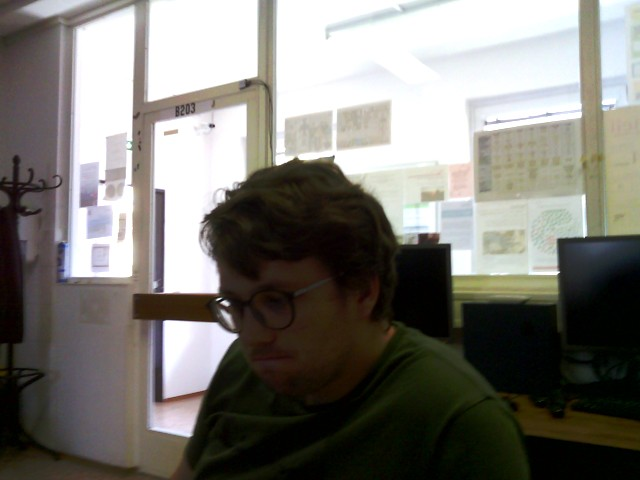
\includegraphics[width=0.72\linewidth]{pics/example_pic_from_pepper.jpg}
\caption{Example of a real image captured by Pepper during testing. The client sends frames of this kind together with robot metadata to the server. The example also illustrates the limited resolution and quality of practical robot-side visual input.}
\label{fig:pepper-client-capture-example}
\end{figure}

Figure~\ref{fig:pepper-client-capture-example} shows an example of the visual input produced by the robot during testing.
%The image is not an offline benchmark image; it is representative of what the client sends from Pepper.
The implementation must handle limited resolution, robot camera exposure, motion, and network transmission rather than assuming a clean image dataset.

The scan action is the wider observation path.
Before scanning, the client records the current head pose.
It then moves the head through configured yaw angles, waits for the head to settle, captures a frame at each pose, and restores the original head pose when configured to do so.
In the current configuration, the scan uses yaw angles around \(-35^\circ\), \(0^\circ\), and \(35^\circ\), but these values are read from \texttt{client\_config.json}.
The captured frames can be sent to the server as one panorama detection request or as separate sequential detection requests.
The panorama request gives the server a wider visual context, while sequential mode preserves each head pose as an independent observation.

Quick look is the fast path for answering ``what do you see?'' with minimal delay.
Panorama scan is the richer path for updating scene memory from multiple viewing directions.
The scan can optionally ask the server for a natural-language summary after detection, but its main purpose is to build a better memory state for subsequent dialogue.

\section{Robot Metadata Sent to the Server}\label{sec:client-metadata}

Every visual request contains image bytes and a metadata object describing the robot state at capture time.
The client sends identifiers for the frame and scan, the capture mode, image dimensions, camera field of view, head pose, body yaw, timestamp, and any available people or social signals.
This is the payload that reaches the server-side perception pipeline; the detailed parsing and fusion are described in Chapter~\ref{chap:server_side_rewrite}.

\section{Server Communication and Local State}\label{sec:client-transport-state}

All server calls go through \texttt{PepperServerTransport}.
Image endpoints use multipart form uploads, while chat, memory, reset, and pregenerated question-answer requests use JSON.
The transport reads endpoint paths and timeouts from configuration.
It also validates the basic response shape before returning data to the turn manager.
For example, caption responses must contain a caption, detection responses must contain an object list, and chat responses must contain a sentence and conversation identifier.

Network and response failures are converted into client-specific exceptions.
Timeouts, unavailable endpoints, and structurally invalid responses are represented by dedicated client errors.
Guarded turn execution catches these errors and speaks localized fallback messages.
The user hears a robot-level failure response instead of raw HTTP details or silence.

The client stores only temporary interaction state.
The local session store remembers the current server conversation id, last caption, last detection timestamp, last scan id, last server response, remembered labels, remembered attributes, remembered relations, and cached question-answer pairs.
It does not own persistent scene memory.
Long-term visual memory and object association remain server responsibilities.
The client mirrors only the parts needed for speech recognition and smooth interaction.

\section{Configuration and Development Modes}\label{sec:client-configuration}

The robot client is configured through its JSON configuration file.
The \texttt{server} section defines the base URL, endpoint paths, timeouts, TLS verification, and whether responses should be published to the dashboard.
The \texttt{capture} section controls camera settings, JPEG quality, scan yaw angles, head movement speed, scan pitch, settle time, and fake camera settings.
The \texttt{dialog} section controls dynamic concept refresh and maximum concept sizes.
The \texttt{panorama}, \texttt{social}, and \texttt{behavior} sections control scan mode, Pepper social-signal collection, acknowledgements, auto-refresh behavior, and retry policy.

Most configuration is read at service startup, which matches normal robot deployment.
The service also exposes selected runtime helpers, such as server URL update, configuration reload, status inspection, and raw speech output.
During testing, these helpers reduce the cost of Pepper's slow deployment cycle.
They do not change the core architecture: QiChat and the tablet still call the same bound service, the service still delegates long actions to the turn manager, and the server remains the owner of grounded perception and memory.

Together, these implementation details complete the robot-side part of the system.
The client provides the embodied interaction layer, while the server provides perception, scene memory, and language reasoning.
The next chapter evaluates the resulting system experimentally, including scene graph generation quality and robot response latency.
